\documentclass{deliverablereport}
\usepackage{wrapfig}
\lstset{stringstyle=\tiny}

\deliverable{UI}{ipython-advanced-interacts}
\deliverydate{31/08/2018}
\duedate{31/08/2018 (M36)}
\author{Odile Bénassy and Nicolas M. Thiéry}

\begin{document}
\maketitle
% This will be the abstract, fetched from the github description
\githubissuedescription

\section{Introduction}

\TODO{Write a one (half) page summary of this introduction, and put it
  in the github description}

The \href{https://jupyter.org}{Jupyter Notebook} is a web application
that enables the creation and sharing of executable documents
containing live code, equations, visualizations and explanatory text.
Reaching far beyond the standard
\href{https://en.wikipedia.org/wiki/Read-eval-print_loop}{REPL}
interaction (Read-Eval-Print Loop), a key feature of Jupyter is its
\href{http://jupyter.org/widgets}{Interactive widgets} which enable
real time interactive data visualizations; the Jupyter community has
developed a large array of widgets for interactive 2D and 3D
visualization of data in the form of charts, maps, tables, etc;
See Figure~\ref{fig:ipyleaflet} for an example, and
\delivref{UI}{vis3d} for ODK's contribution to 3D visualization.
Furthermore, widgets can be \emph{composed} to build rich
applications, with all the usual UI components (e.g. menus, sliders,
or layout control).

\begin{figure}[h]
  \begin{center}
    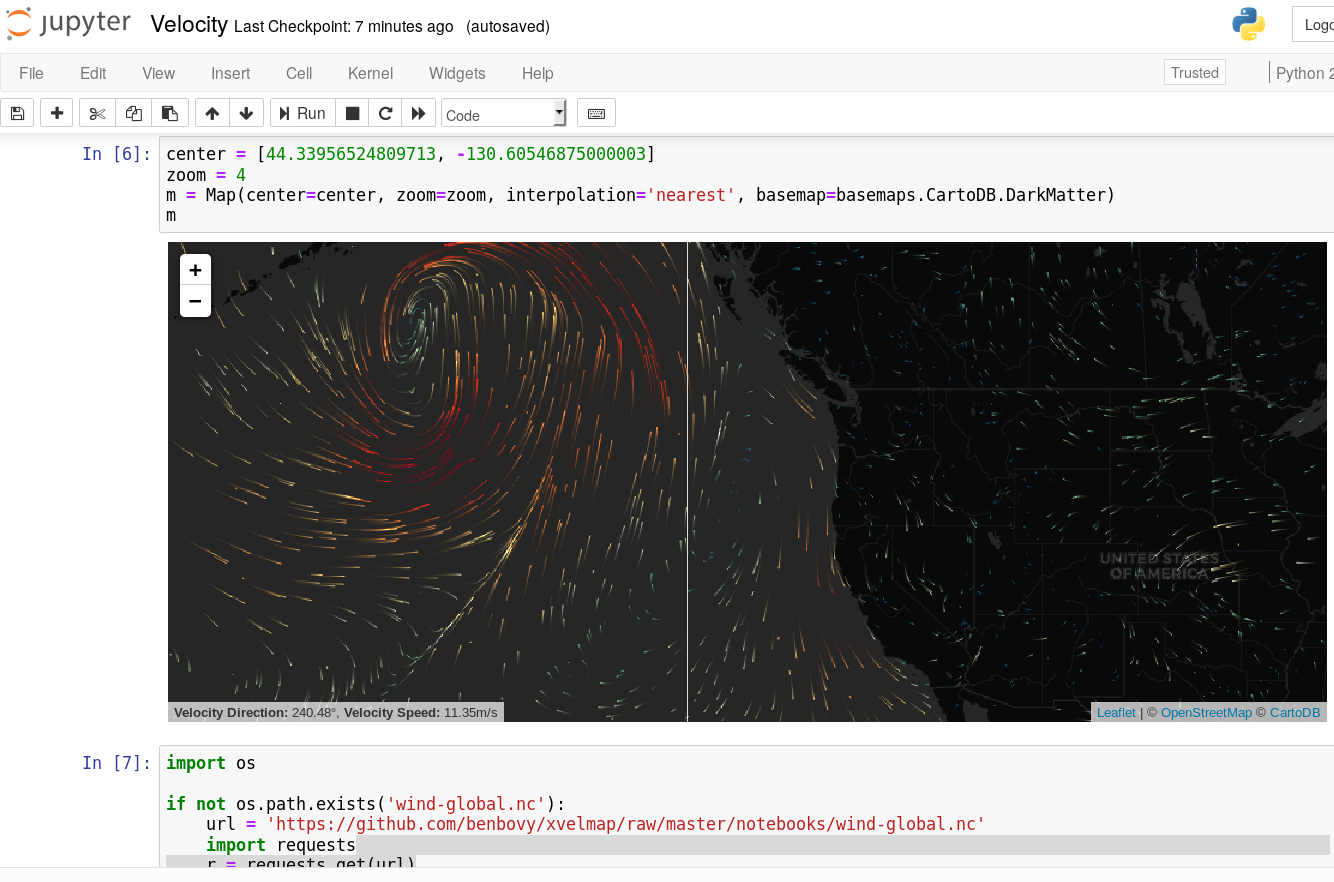
\includegraphics[width=\textwidth]{images/Velocity}
  \end{center}
  \caption{A Jupyter widget displaying an interactive map based on
    OpenStreetMap data, overlayed with a visualisation of wind velocity
    data (courtesy of the \lstinline{ipyleaflet} documentation).}
  \label{fig:ipyleaflet}
\end{figure}

\TODO{screenshot: some Jupyter based web application}

Hence, the Jupyter stack provides a very flexible environment catering
for use cases ranging from a novice users typing just a few commands
or browsing interactive documents to more advanced users authoring
rich interactive applications for their fellows.

The question we are tackling in this report is how this technology --
and specifically Jupyter widgets -- can be leveraged for pure
mathematics. The unique challenge comes from the huge variety of
mathematical objects that the user may want to visualize and
interact with, and the variety of graphical representations;
see Figure~\ref{fig:math_viz} for some examples.

%\newpage

\begin{figure}%[h]
  \begin{center}
    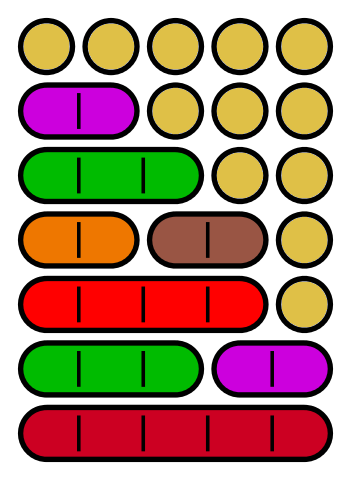
\includegraphics[width=0.20\textwidth]{images/partitions-of-5}
    \hfil\hfil
    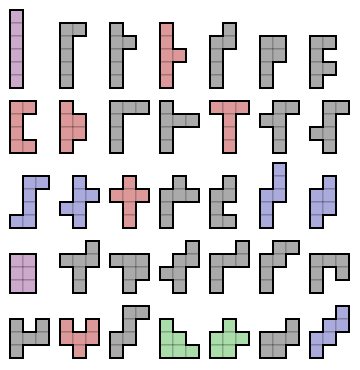
\includegraphics[width=0.25\textwidth]{images/hexominoes}
    \hfil
    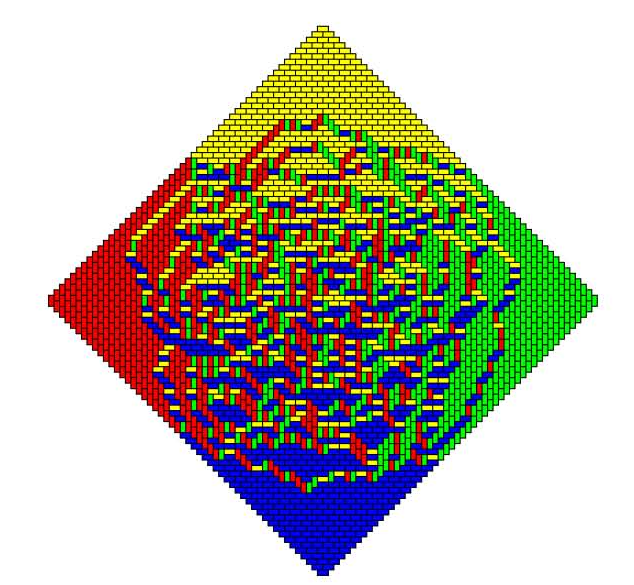
\includegraphics[width=0.30\textwidth]{images/AztecDiamond}
%   \end{center}
% \end{figure}
% \begin{figure}[h]
%   \begin{center}
    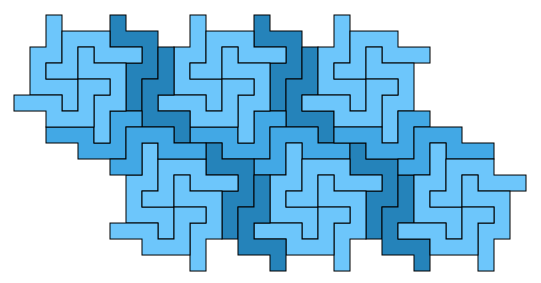
\includegraphics[width=0.4\textwidth]{images/nonominoes}
    \hfil
    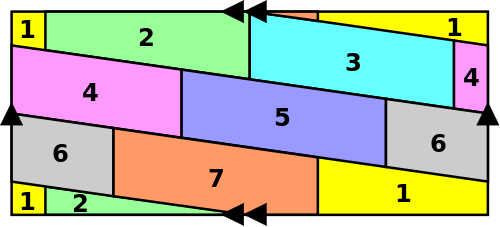
\includegraphics[width=0.4\textwidth]{images/500px-Torus_with_seven_colours}
%   \end{center}
% \end{figure}
% \begin{figure}[h]
%   \begin{center}
    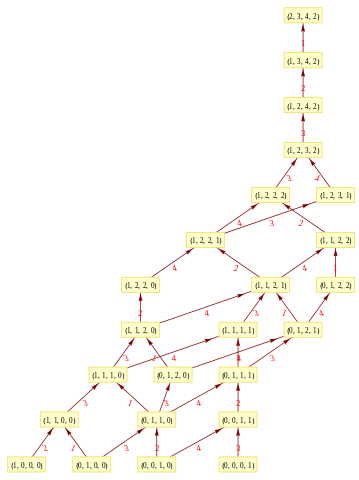
\includegraphics[width=0.3\textwidth]{images/359px-F4HassePoset}
    \hfil
    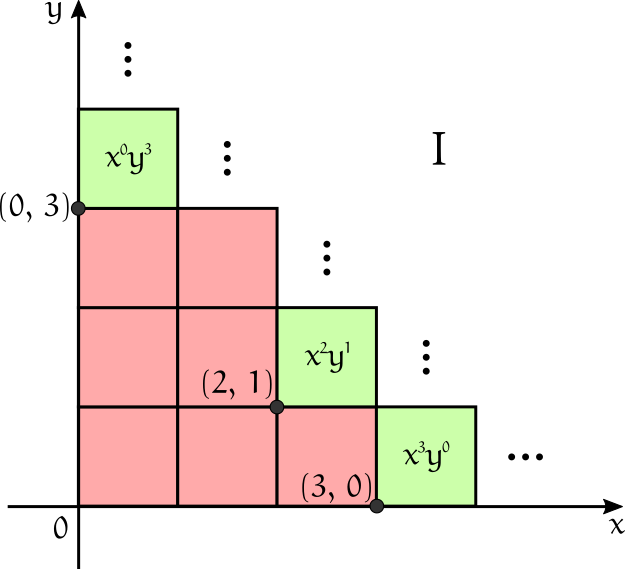
\includegraphics[width=0.3\textwidth]{images/Wikipic}
    \hfil
    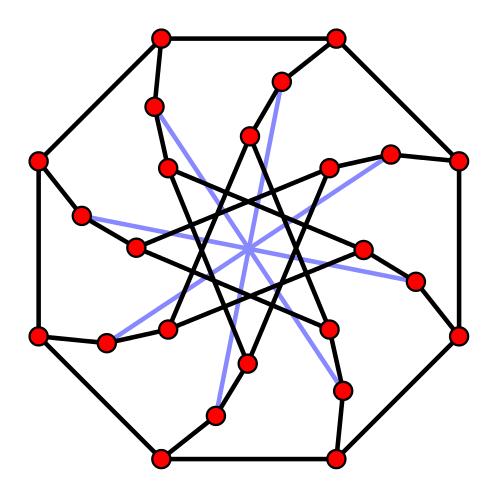
\includegraphics[width=0.3\textwidth]{images/500px-McGee_graph}
%   \end{center}
% \end{figure}
% \begin{figure}[h]
%   \begin{center}
    
\includegraphics[width=0.3\textwidth]{images/fractioncont}
    \hfil
    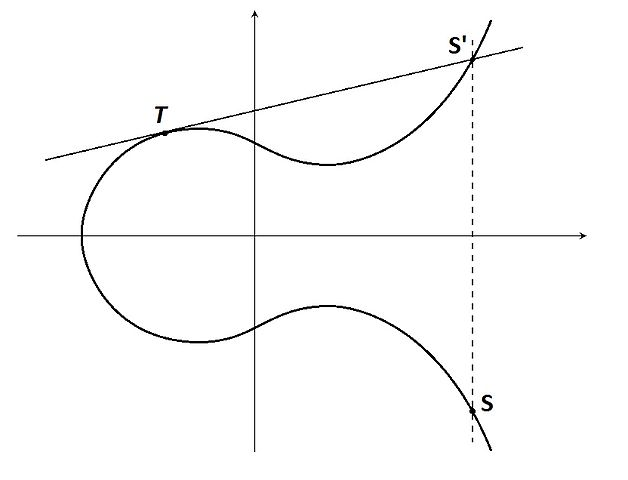
\includegraphics[width=0.3\textwidth]{images/elliptic-curve}
    \hfil
    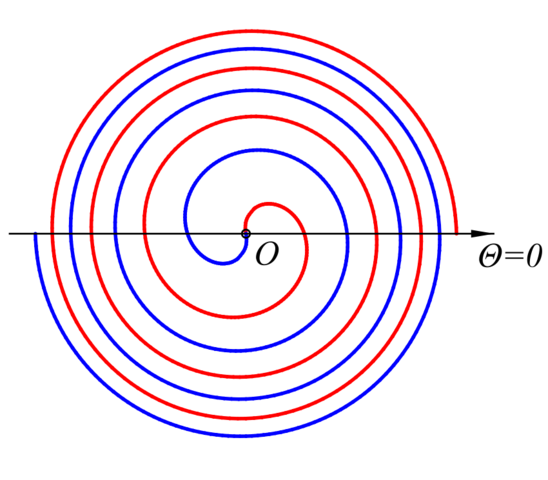
\includegraphics[width=0.3\textwidth]{images/548px-Fermat's_spiral_01}
%   \end{center}
% \end{figure}
% \begin{figure}[h]
%   \begin{center}
    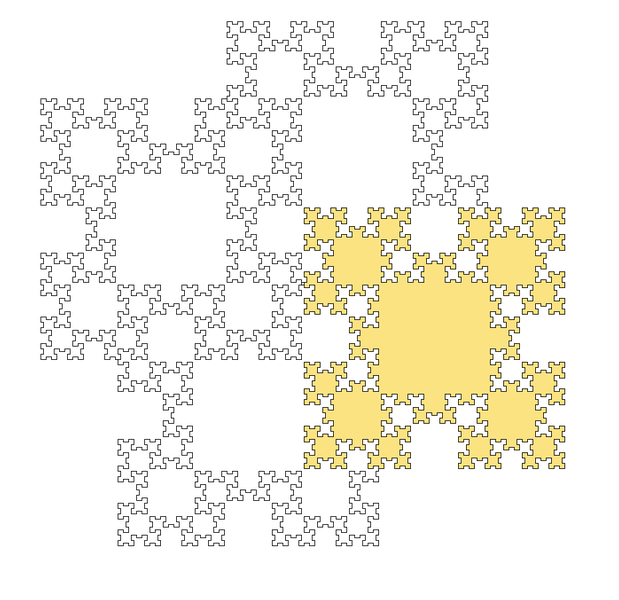
\includegraphics[width=0.3\textwidth]{images/619px-Tiling_Fibonacci_word_fractal}
    \hfil
    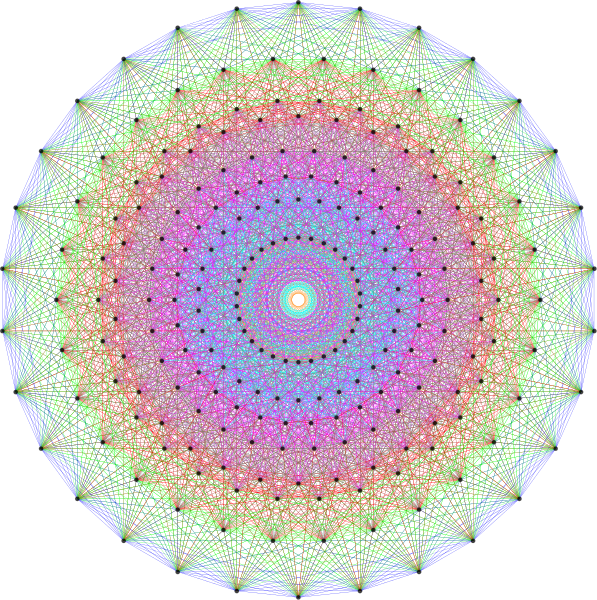
\includegraphics[width=0.3\textwidth]{images/597px-E8Petrie}
  \end{center}
  \caption{Some graphical visualizations of mathematical objects}
  \label{fig:math_viz}
\end{figure}

%\TODO{search on wikipedia for a nice collection of pictures: a
%  partition, a polyomino, an aztec diamond, a monomial ideal, a graph,
%  a poset, a formula - fraction continue, a curve, ...}. diagramme de Venn ; th des 4 couleurs sur une carte mathématique

We therefore can't hope to provide hand crafted solutions for each
situation; instead we need to devise a toolbox of generic solutions
from which users can easily derive specialized visualizations for
their own pet objects.

In this report, we pursue two directions.

In Section~\ref{section:combi}, we explore the development of widgets
for the graphical visualization in combinatorics -- or more generally
discrete mathematics. The choice of this area of mathematics was, to
some extent out of personal interest and expertise, but more
importantly because devising good representations -- mental images --
of discrete objects is at the heart of research in combinatorics. We
start by reviewing in Section~\ref{section:francy} the GAP package
\href{https://github.com/mcmartins/francy}{Francy} which currently
explores the natural use case of objects that admit a graph-like
representation: trees, graphs, lattices of subgroups, crystals,
posets, discrete markov chains, just to name a few. At this stage, ODK
has a light contribution to the development of this package, through
the supervision(?) of ODK's member Markus Pfeiffer. We highlight the
lessons learned there and describe upcoming collaboration toward
bringing Francy\'s features to SageMath.

Then, in Section~\ref{section:grid}, we report on the implementation
in SageMath of a generic widget for objects that admit a
representation as a collection of cells on a 2D grid, and
specializations for typical objects such as partitions, tableaux,
polyominos, aztec diamonds, mazes. One aspect which we explore beyond
Francy is not only \emph{interactive visualization} but also
\emph{interactive edition}, where the underlying mathematical object
gets changed by the user gestures. This is the occasion to explore the
flexibility of the the design patterns emerging from Francy.

The choice of this use case was motivated by two important features:
\begin{itemize}
\item the visualization part is relatively simple making it a good
  case for prototyping;
\item the potential impact is high due to the large number of objects
  covered, bringing in opportunities for testing how users manage to
  to adapt our generic tools for their own pet objects;
\end{itemize}

In a second direction, we explore in
Section~\ref{section:sage-explorer} the use of Jupyter widgets not only
for the graphical visualization of an object, but for displaying a
page offering a synthetic overview of the information about that
object, including type, important properties and invariants, available
operations, related objects, documentation, etc. All sort of
information that is readily available by introspection but that a UI
can make easy to discover and emphasize according to relevance. The
challenge is that, given the huge variety of objects in a system like
SageMath, we can't afford to hand craft such pages for each type of
objects. We report on our prototype
\lstinline{sage-explorer} that exploits the semantic embedded into the
system to produce a reasonable overview page automatically tailored to
each object.

\TODO{Screenshot of Sage-explorer?}

Altogether, the Jupyter Widget technology has proven as mature and
flexible as we hoped for. Designing new widgets does take some
expertise, but from the experience we gained, we are confident that it
lends itself well to the implementation of generic widgets by power
users that can be specialized by casual users and used by novices.

Three main challenges arise along the way which we will continue to
explore and tackle during the last year of OpenDreamKit:
\begin{itemize}
\item Implementing visualization widgets is time consuming and
  requires specific expertise that developers of computer algebra
  systems usually don't have. It's therefore desirable to reuse them
  across mathematical objects that share a certain type of
  visualization, and across computer algebra systems. How to best
  design widgets to decouple them from the specific objects or
  programming language at hand?
\item User interface and visualization technologies tend to evolve
  much faster than computational systems; how to best design widgets
  to decouple the semantic part of the visualization of the widgets
  from the actual visualization technology, in order to prepare for a
  smooth and cheap migration path when such technology evolves and
  foster long term sustainability?
\item Widgets, as all modern web technologies, rely a lot on
  asynchronous execution. This is quite a different model from the
  Read-Eval-Print main loop that many not-so-young computational
  systems (including SageMath!) have originally been designed for, and
  such systems don't always behave well under asynchronous pressure:
  we have faced some bad crashes. How deep is the difficulty? How hard
  will it be to resolve it?
\end{itemize}

\section{State of the art}

\TODO{A standalone section? Or comments about it in the intro and along the way?}

In addition to the interactive widgets already delivered with ipywidgets (e.g. Sliders), numerous investigations, towards these goals, have been conducted in mathematical environments.

\begin{itemize}
\item The \href{http://www.lmfdb.org/}{LFMDB} database displays a comprehensive view of L-functions and Modular Forms in a web browser, yet misses manipulation possibilities on the objects.
\item In the \href{https://core.ac.uk/download/pdf/9839511.pdf}{The
  Larch Environment} document (2013), Geoffrey W. French presents his own graphical
  interactive programming environment called \emph{larch}.
  One of his main ideas is to
  \emph{coerce} objects into graphical representations. Meaning that
  every object must know how it can be graphically represented, this
  representation being the default one and can be tailored by the
  user: G.W. French speaks of different \emph{perspectives} for the
  same object. The Larch Environment also maintains a state of objects
  in order to automatically refresh the representation.
  However, the Larch environment is designed to run locally, i.e. not
  within any browser, and the project was discontinued in 2014.
\end{itemize}

\section{Interactive visualization of combinatorial objects}
\label{section:combi}

\subsection{Francy: an Interactive Discrete Mathematics Framework for GAP}
\label{francy}

Francy is a package for interactive visualisation in discrete
mathematics. It's developed mainly by Manuel Martins, with supervision
by ODK's member Markus Pfeiffer. For now, Francy has been focusing on
the interactive visualisation of objects that admit a graph-like
representation (trees, graphs, ...). Features include for example
zoom-and-pan, moving nodes, clustering, menus for
activating/deactivating interactions, etc. Those are basic interactive
graph drawing features and are not particularly impressive by
themselves: after all, interactive graph drawing and editing has been
the subject of a whole community, with series of conferences such as
the \emph{International Symposium on Graph Drawing and Network
  Visualization}, and acclaimed tools like \lstinline{graphviz} or
\lstinline{tulip}. What makes Francy stand is to bring those feature
to computational systems and, more importantly, explore how to best
leverage the technology to empower users of such systems to adapt it
to their needs.

\TODO{somewhere: macaulay's package}

At this stage, Francy is a package for the GAP computer algebra
system. However its features would be extremely valuable for other
systems and in particular \Sage. Also Francy uses Jupyter Widgets as
GUI framework and \href{d3js.org}{D3JS javascript library} library for
visualisation. %which manipulates the browser DOM for the graphical display itself
While those are flourishing technologies that are promising for the
years to come, lessons learned the hard way from the past (e.g. within
the xgap project) shows that, at the scale of decades, GUI and
visualization frameworks change at a faster pace than computational
systems and visualization needs.

To tackle these two tensions, Francy has taken the approach of
decoupling itself from the computational system and from the GUI
framework and visualization libraries. It does this by introducing an
intermediate layer of semantic models of what graphical
representations are. With this approach, integrating a new
computational system reduces to providing a backend describing the
desired graphical representations for its mathematical objects in the
semantic model. Similarly, integrating GUI framework reduces to
providing a frontend describing how to concretely render and interact
with the graphical representations from the model. In practice, the
semantic model takes the form of an intermediate JSON data format,
with JSON data being passed from the computational system to the
browser.

%\subsection{Francy, }

\TODO{Time permitting: a picture of the data flow}


\subsection{A generic widget for objects with a grid-like representation}
\label{grid}

We have seen a \emph{design pattern} emerging in the previous section:
without this being formalized, a similar approach had been taken in
Sage for static graph drawing, using the so-called ``dot'' format of
the graphviz project as intermediate data format, to later produce
graph pictures in a variety of formats (latex, pdf, svg).

Similarly, in the
\href{http://mupad-combinat.sourceforge.net}{MuPAD-Combinat} project a
generic intermediate data format was designed for all objects that can be
drawn by filling out certain cells in a 2-dimensional grid. Here is,
for example, a drawing of \emph{skew tableau}, an important kind of
combinatorial object arising in representation theory:

\begin{wrapfigure}{r}{0.25\textwidth}
    \begin{center}
      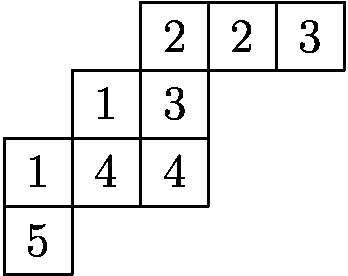
\includegraphics[width=100px]{images/JDTSlide}
      %\caption{A grid widget}
\end{center}
\end{wrapfigure}
We will call such a drawing a \emph{grid-like representation}.

From the intermediate data format, drawings could be produced in a
variety of format: latex, pdf, various forms of ascii art, ...; see
\href{http://mupad-combinat.sourceforge.net/doc/en/Cat_Combinat/CombinatorialClassWith2DBoxedRepresentation.html}{Combinatorial Class With 2DBoxedRepresentation}.
This achieved the same two levels of decoupling as we have seen in Francy.

We decided to build on this previous experience to explore not only
drawing, but also \emph{interactive editing}: here, the interaction
not only affects the visualization, but also induces changes to the
the original mathematical objects via the intermediate data format.
Thus the data flow is now bidirectional.
\TODO{Time permitting: a picture of the bidirectional data flow}

Technically speaking, we aimed for the implementation of a generic
Jupyter widget meant for all SAGE-objects admitting a grid-like
representation.

\TODO{NT: additional challenge: the interaction requires richer
  messages where not only data representing the, but also questions
  are asked (validity, valid changes, ...) + temporary invalidity. }.

This use case combined several advantages:
\begin{itemize}
\item The UI part was relatively straightforward, for example
  requiring no Javascript side extension;
\item Little mathematical background was required; this, together with
  the previous point, made for a smooth learning curve for our
  Research Software Engineer;
\item It was a low hanging fruit with a large coverage;
\item The end result is immediately useful to colleagues, enabling
  early feedback from users;
\item There is a large variety of potential specializations, each with
  it's own quirks and specifics.
\end{itemize}
Hence, this use case provided a unique challenge: all the difficulty
resided in the the design of a generic solution that encapsulates as
much of the technicalities as possible, enabling users to specialize
the generic solution for their own pet objects with little expertise.

\subsection{Description of the design, of the API that subclasses must
  implement, code examples}

\begin{figure}[h]
  \begin{center}
    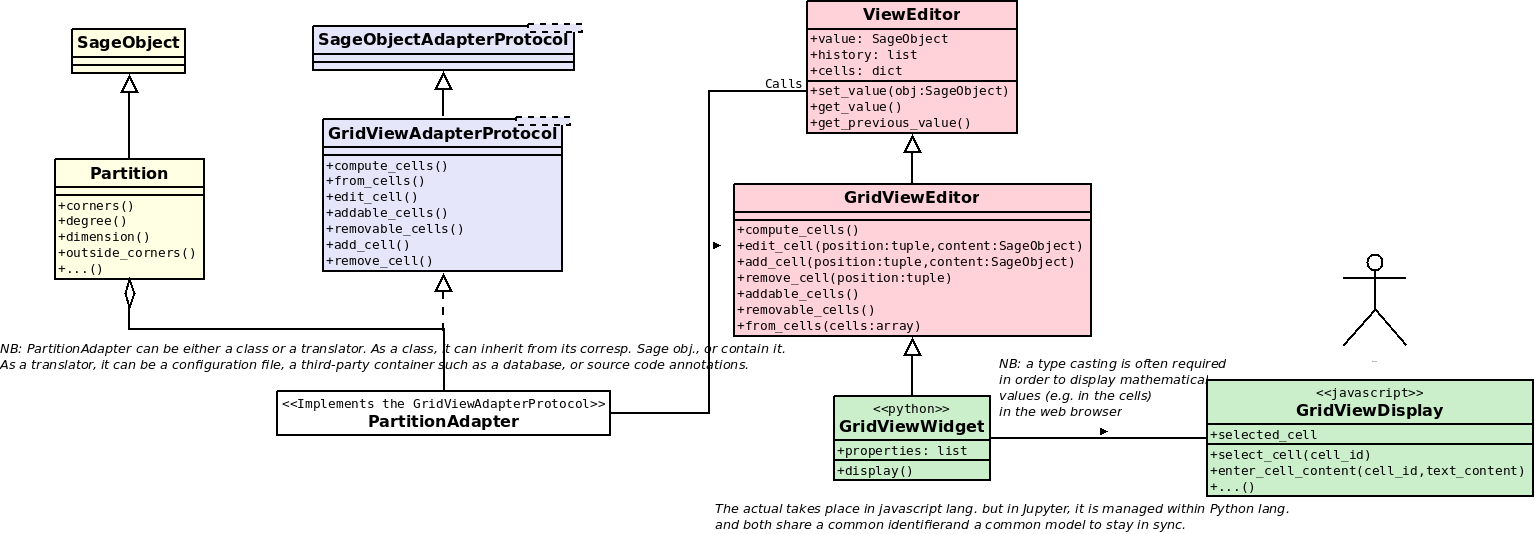
\includegraphics[width=\textwidth]{schemas/SageViewEditor}
  \end{center}
  \caption{Sage View Editor classes}
  \label{fig:lmfdb}
\end{figure}

We have developped a \emph{GridViewWidget} for representing - and
interacting with - Sage Objects in Jupyter environment, in a browser.

The interaction possibilities currently are the following:
\begin{itemize}
  \item editing a cell content
  \item adding or removing cells
  \item selecting cells for more interactions
\end{itemize}

This \emph{GridViewWidget} is based on a \emph{GridViewEditor}, that
is GUI-agnostic.

\emph{GridViewEditor} can operate in various Sage grid-representable objects like graphs,
matrices, or tableaux. As it needs to operate on each in the same way,
and in effect they have various method names, or signatures, or
different features, we felt the need to define a list a methods to be
implemented by them, i.e. an \emph{API}.

Currently hidden in the \emph{GridViewEditor} itself, we intend to promote
the development of adapters for the Sage objects, either by implementing Adapter
classes as such, or by writing translating information. Here are a few code examples
for both strategies:

\begin{lstlisting}
class GenericGraphGridViewAdapter(GenericGraph):
  ...
  def from_cells(self, cells={}):
    g = GenericGraph()
    g.add_vertices(list(cells.keys()))
    return g

class PartitionGridViewAdapter(Partition):
  ....
  def add_cell(self, coord):
    return self.add_cell(self.coord[0], self.coord[1])

class StandardTableauGridViewAdapter(StandardTableau):
  ....
  def from_cells(self, cells={}):
      positions = sorted(list(cells.keys()))
      try:
        return StandardTableau([[cells[pos] for pos in positions if pos[0]==i] for i in uniq([t[0] for t in positions])])
      except:
      raise TypeError("Cannot generate a valid StandardTableau!")
\end{lstlisting}

Second strategy: a translator can be written directly in the source
code, with \emph{Python annotations}:

\begin{lstlisting}
@grid_view_adapter(\{addable_cells:self.shape().addable_cells, removable_cells:removable_cells\})
class StandardTableau:
  /.../
\end{lstlisting}

%The users can specify their own tile shape. For example they can
%use \emph{IPyWidgets} buttons or text inputs.

\subsection{Potential applications}

\begin{wrapfigure}{r}{0.25\textwidth}
    \begin{center}
      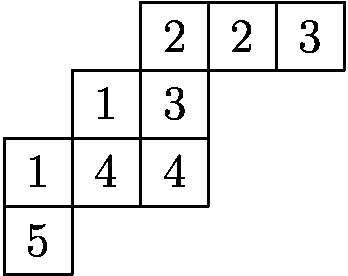
\includegraphics[width=100px]{images/JDTSlide}
      %\caption{A tableau widget}
\end{center}
\end{wrapfigure}

Grid-like representable objects cover many algebraic or combinatoric
objects: matrices, partitions, grid graphs, tableaus, ribbons ..

Apart from displaying and editing an object, more possibilities can be
imagined

\begin{wrapfigure}{r}{0.25\textwidth}
    \begin{center}
      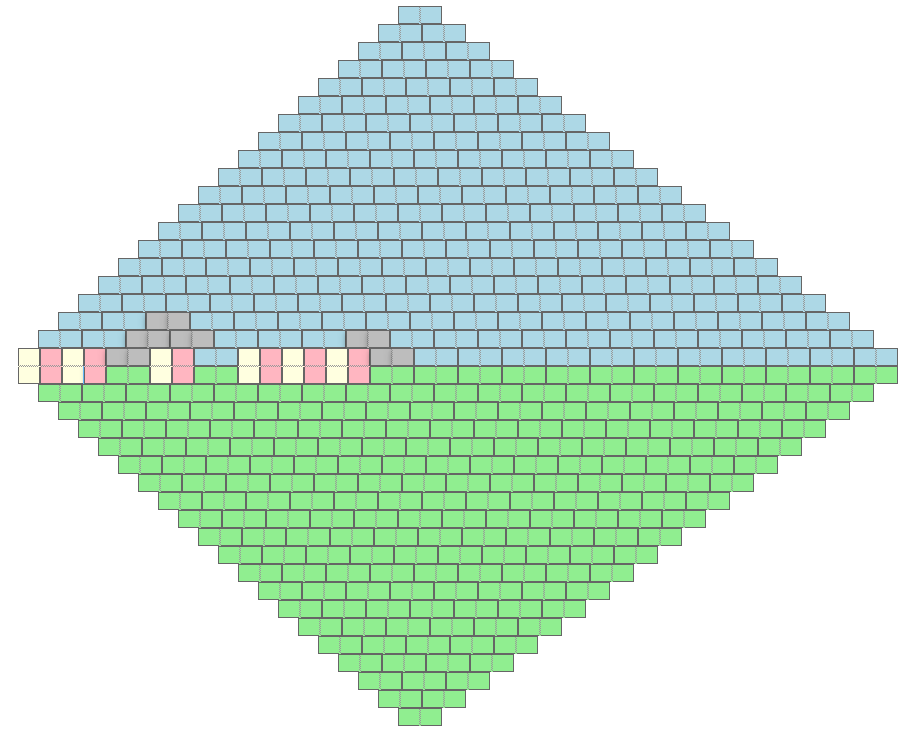
\includegraphics[width=100px]{images/dominos-azteque}
      %\caption{A tableau widget}
\end{center}
\end{wrapfigure}

As an example, we have developed a domino-like representation of
\emph{grid-graph matchings} with a \emph{flipping} feature on neighboring dominos.

The code is distributed as a Sage package
\href{https://github.com/sagemath/sage-combinat-widgets/}{sage-combinat-widgets}
which is meant to grow beyond this initial seed, attracting
contributions from the community, and presumably be integrated
progressively into SageMath.

\subsection{Strategy to get feedback from users}

\begin{itemize}
  \item Attending local seminars at \emph{Laboratoire de Recherche Informatique} or/and \emph{\href{https://www.lix.polytechnique.fr/}{Laboratoire d'Informatique de l'École Polytechnique}}
  \item Release some implementation examples for a few object types ; write a tutorial on how to write your own ; invite users to write feedback, either on the development mailing list, or on the  project \emph{sage-combinat-widgets} issues interface
  \item Take advantage on the next SAGE-days to organize a dedicated workshop and collect direct feedback there
\end{itemize}

\subsection{Future plans}

In the upcoming year, we plan to collaborate tightly with Francy to:
\begin{itemize}
\item Bring Francy's features to \Sage by implementing a backend. This
  would finally bring a solution to a long time yet pressing need of
  the community that was so far only partially fulfilled by
  unsustainable prototypes like Sage's
  \href{http://doc.sagemath.org/html/en/reference/graphs/sage/graphs/graph_editor.html}{graph editor}.
\item Further explore the design pattern with over kinds of graphical
  representations (starting from the grid view representation of the
  next section), with a similar decoupling between a Sage backend, a
  semantic model, and a Jupyter/JS frontend.
\item Contribute the models and frontends to Francy, making the
  features available to GAP.
\end{itemize}

\section{Sage-explorer}
\label{section:sage-explorer}

\TODO{tension SAGE/javascript concernant l'emplacement des appels de
  méthodes}

\subsection{Sage-explorer should be as rich as LMFDB, and is interactive}

\begin{figure}[h]
  \begin{center}
    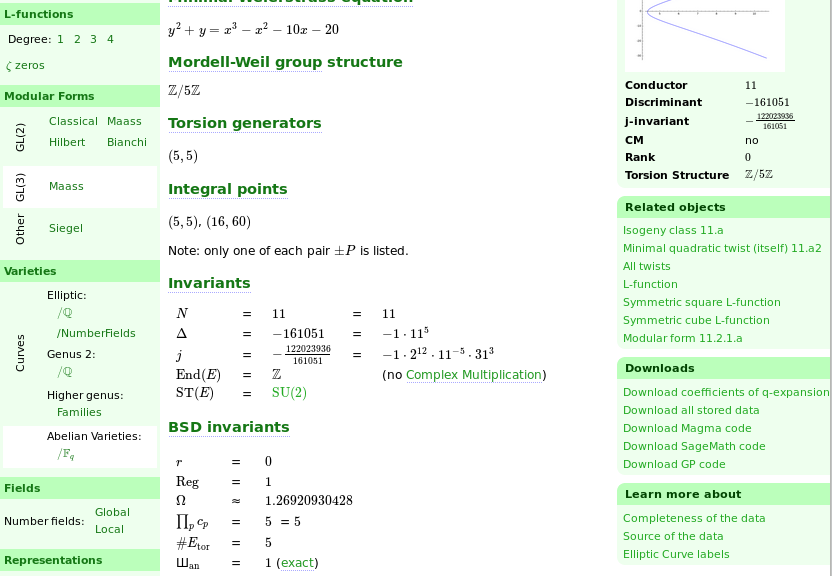
\includegraphics[width=\textwidth]{images/LMFDB-11a2}
  \end{center}
  \caption{L-fonctions database on elliptic curve ``11a2''}
  \label{fig:lmfdb}
\end{figure}

\TODO{Comparative screenshot of the same curve in sage-explorer}

In LMFDB, many methods results are calculated at page opening, while
with Sage Explorer, the calculation is run only on demand, except for
some widely used \emph{properties}.

\TODO{A bunch of screenshots}

\subsection{Overview}

Sage-explorer comprises:

\begin{itemize}
  \item A block made of a title and a list of properties for the object
  \item A graphical representation of the object
  \item A list of object methods
  \item A panel for documentation and computations
\end{itemize}

We wanted to make available key information at once and, apart from
that, let the user run the methods they like.

This is why we select only some of the methods, the results of which
are called \emph{properties} and are configurable.

\TODO{Example configuration source code}

The object graphical representations try to be as ``natural'' as
possible for the user. So we use plotting when relevant. For
combinatorial objects, we call the \emph{sage-combinat-widgets}
package. As soon as integration is made with the \emph{sage-combinat-widgets},
the graphical representation will mirror the object changes in real
time, too.

The widget choice is also specified in the configuration. Yet we
intend to make it available directly within Sage source code, thanks
to \emph{Python annotations}.

Sage object methods are listed in the menus to facilite
discovering, alphabetically ordered. As method lists can be very long,
we have split them according to the class where they appear in Sage source
code and we intend to find more than one categorization way.

When a method is selected, its documentation and signature are made
available. The user can then fill out the argument and run the method
to get a result.

Finally, links appear in many places in the explorer. Clicking on one
of those links opens a new object in the explorer.

\subsection{Configuration and semantics}
\label{semantics}

Three configuration files specify:

\begin{itemize}
\item Graphical display widgets associated to Sage objects
  \item Properties associated to Sage objects, i.e. which object methods are
    to be considered as object properties.
\item The objects lists (or \emph{catalogs}) for the Explorer Index
\end{itemize}

To specify these, especially the first two, a set of logical rules
have been defined, are implemented in YAML syntax and parsed by the
Sage-explorer code.

In the future, we expect to get all this semantic information, or part of it,
written directly in Sage source code.

This could take the form of \emph{private attributes} or \emph{annotations}, like:

\begin{itemize}
\item a \emph{\_widget\_} attribute specified in Sage categories source files
\item specific annotations, using \emph{@} Python syntax for annotations
  \end{itemize}

Where will still remain, for the user, the possibility of overloading
the widget class - \emph{\_widget\_} being only the default) and
specify which of the \emph{properties} she wants to get rendered in effect.

Hence, there will be a contiuum between semantic written in Sage
source code and configuration files, taking into account semantic
information, logical rules specifying how to read this semantics, and
parametrization by the user, given that (for \emph{properties}:

\begin{itemize}
\item some semantics can be specified as object attributes: ``is this method a
  property?'' and
  \item ``is this property worth rendering by default?''  while we
    still have to decide
  \item ``is computing this property not going to slow down the display?''
\end{itemize}

\subsection{Upcoming work}

\begin{itemize}
\item develop interactivity for some methods in the widgets
\item tutorial: how to build a widget
\item enhance explorer index
\end{itemize}

\subsection{Strategy to get feedback from users?}

\TODO{See above (ou bien on recopie dès que c'est bien fixé)}

\appendix

\TODO{The demo notebooks?}



\end{document}

%%% Local Variables:
%%% mode: latex
%%% TeX-master: t
%%% End:

